\documentclass[11pt,aspectratio=169]{beamer}
\usepackage{amsmath,amssymb,bm,booktabs,tikz}
\usetikzlibrary{arrows.meta,calc}
\usetheme{default}
\setbeamertemplate{navigation symbols}{}
\setbeamertemplate{headline}{}
\setbeamertemplate{footline}{%
  \leavevmode\hbox{%
    \begin{beamercolorbox}[wd=\paperwidth,ht=2.6ex,dp=1.1ex,right]{page number in head/foot}%
      \insertframenumber/\inserttotalframenumber\hspace{0.35cm}
    \end{beamercolorbox}}}
\setbeamertemplate{frametitle}{\vspace{0.25cm}\insertframetitle\par\vspace{0.08cm}\hrule}
\setbeamercolor{normal text}{fg=black,bg=white}
\setbeamercolor{frametitle}{fg=black,bg=white}
\setbeamercolor{structure}{fg=black}
\setbeamersize{text margin left=0.7cm,text margin right=0.7cm}
\definecolor{femblue}{RGB}{47,99,143}
\definecolor{femorange}{RGB}{198,91,42}
\newcommand{\bu}{\bm u}
\newcommand{\bv}{\bm v}
\newcommand{\bw}{\bm w}
\newcommand{\bF}{\bm F}
\newcommand{\bP}{\bm P}
\newcommand{\bI}{\bm I}
\newcommand{\bb}{\bm b}
\newcommand{\bt}{\bm t}
\newcommand{\bX}{\bm X}
\newcommand{\bU}{\bm U}
\newcommand{\bR}{\bm R}
\newcommand{\bK}{\bm K}
\newcommand{\Grad}{\operatorname{Grad}}
\newcommand{\Vzero}{\mathcal V_0}
\newcommand{\Vhzero}{\mathcal V_{h,0}}
\DeclareMathOperator{\tr}{tr}
\DeclareMathOperator{\diag}{diag}

\begin{document}

\begin{frame}
\centering\vfill
{\LARGE\bfseries Nonlinear Finite Element Methods\par}
\vspace{0.5cm}
{\Large Lecture 2: Newton Iteration and the Tangent System\par}
\vspace{0.5cm}
Prashant K. Jha\par
ME/BME 736\par
November 5, 2026
\vfill
\end{frame}

\begin{frame}{Lecture outline}
\begin{enumerate}
\item Total potential energy, its variations, and the residual.
\item Newton's method for a scalar equation.
\item Linearization of the hyperelastic variational residual.
\item Finite element residual, tangent matrix, and correction boundary data.
\item A stretch example and checks on the nonlinear solve.
\end{enumerate}
\vspace{0.3cm}
The aim is to obtain the linear system solved at each Newton iteration,
including its entries and its right-hand side.
\end{frame}

\begin{frame}{Recall: the hyperelastic residual}
On the fixed reference body, $\bF(\bu)=\bI+\Grad\bu$ and
$\bP=\partial\Psi/\partial\bF$.
With prescribed reference loads independent of displacement,
\[
\begin{aligned}
a_{\rm hyp}(\bu;\bv)
&=\int_{\Omega_0}\bP(\bF(\bu)):\Grad\bv\,\mathrm dV_0,\\
\ell_{\rm hyp}(\bv)
&=\int_{\Omega_0}\bb_0\cdot\bv\,\mathrm dV_0
+\int_{\Gamma_{0t}}\overline{\bt}_0\cdot\bv\,\mathrm dA.
\end{aligned}
\]
Our starting equation is
\[
\boxed{R(\bu;\bv)=\ell_{\rm hyp}(\bv)-a_{\rm hyp}(\bu;\bv)=0
\quad\forall\bv\in\Vzero.}
\]
Here $\bu=\overline{\bu}$ on $\Gamma_{0u}$, while every
$\bv\in\Vzero$ is zero there. We seek an admissible deformation with
$\det\bF>0$. A trial displacement generally has a nonzero residual.
\end{frame}

\begin{frame}{Total potential energy and the variational problem}
With prescribed reference loads independent of displacement, define
\[
\Pi_{\rm hyp}(\bu)
=\int_{\Omega_0}\Psi(\bF(\bu))\,\mathrm dV_0
-\ell_{\rm hyp}(\bu).
\]
For $\bv\in\Vzero$, use
$\bF(\bu+\epsilon\bv)=\bF(\bu)+\epsilon\Grad\bv$ and
$\bP=\partial\Psi/\partial\bF$. The first variation is
\[
\begin{aligned}
\delta\Pi_{\rm hyp}(\bu;\bv)
&=\left.\frac{\mathrm d}{\mathrm d\epsilon}
\Pi_{\rm hyp}(\bu+\epsilon\bv)\right|_{\epsilon=0}\\
&=\int_{\Omega_0}\bP(\bF(\bu)):\Grad\bv\,\mathrm dV_0
-\ell_{\rm hyp}(\bv)\\
&=a_{\rm hyp}(\bu;\bv)-\ell_{\rm hyp}(\bv)=-R(\bu;\bv).
\end{aligned}
\]
Thus stationarity is exactly the original variational problem:
\[
\boxed{\delta\Pi_{\rm hyp}(\bu;\bv)=0\ \forall\bv\in\Vzero
\quad\Longleftrightarrow\quad
a_{\rm hyp}(\bu;\bv)=\ell_{\rm hyp}(\bv)\ \forall\bv\in\Vzero.}
\]
A stationary point need not be a minimum.
\end{frame}

\begin{frame}[fragile]{Second variation and the residual derivative}
For twice-differentiable $\Pi_{\rm hyp}$ and fixed $\bv,\bw\in\Vzero$, define
\[
\delta^2\Pi_{\rm hyp}(\bu;\bv,\bw)
:=\left.\frac{\mathrm d}{\mathrm d\epsilon}
\delta\Pi_{\rm hyp}(\bu+\epsilon\bw;\bv)\right|_{\epsilon=0}.
\]
Since $R(\bu;\bv)=-\delta\Pi_{\rm hyp}(\bu;\bv)$,
\[
\begin{aligned}
\delta_uR(\bu;\bv)[\bw]
&=\left.\frac{\mathrm d}{\mathrm d\epsilon}
R(\bu+\epsilon\bw;\bv)\right|_{\epsilon=0}\\
&=-\left.\frac{\mathrm d}{\mathrm d\epsilon}
\delta\Pi_{\rm hyp}(\bu+\epsilon\bw;\bv)\right|_{\epsilon=0}\\
&=-\delta^2\Pi_{\rm hyp}(\bu;\bv,\bw).
\end{aligned}
\]
In UFL, \texttt{u} is the current displacement, \texttt{v} the test
function, and \texttt{w} the trial direction:
\begin{verbatim}
residual = -ufl.derivative(Pi, u, v)
tangent = ufl.derivative(residual, u, w)
\end{verbatim}
\end{frame}

\begin{frame}{Newton's method: one scalar equation}
Consider $r(z)=z^2-2=0$. Let $z^k$ be an approximation and
$\Delta z^k$ its correction.
Linearize about $z^k$:
\[
r(z^k+\Delta z^k)
\approx r(z^k)+r'(z^k)\Delta z^k.
\]
Set this linear approximation to zero:
\[
\boxed{r'(z^k)\Delta z^k=-r(z^k),\qquad
z^{k+1}=z^k+\Delta z^k.}
\]
Starting from $z^0=1$,
\[
r(1)=-1,\qquad r'(1)=2,\qquad
2\Delta z^0=1,\qquad z^1=1.5.
\]
Each iteration solves a linear correction equation and updates the approximation.
\end{frame}

\begin{frame}{A tangent equation predicts the next approximation}
\begin{columns}[c,onlytextwidth]
\begin{column}{.62\textwidth}
\centering
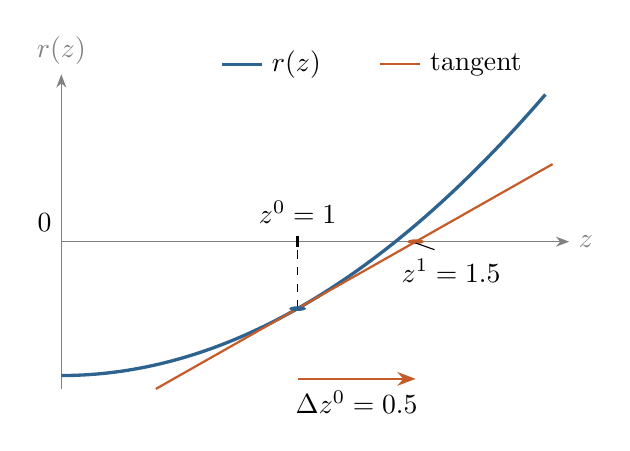
\begin{tikzpicture}[>=Stealth,xscale=3,yscale=.85]
\draw[->,gray] (0,0)--(2.15,0) node[right] {$z$};
\draw[->,gray] (0,-2.2)--(0,2.5) node[above] {$r(z)$};
\node[above left] at (0,0) {$0$};
\draw[very thick,femblue,domain=0:2.05,samples=90]
  plot(\x,{\x*\x-2});
\draw[thick,femorange,domain=.4:2.08] plot(\x,{2*\x-3});
\draw[dashed] (1,-1)--(1,0);
\fill[femblue] (1,-1) circle(1pt);
\draw[thick] (1,.08)--(1,-.08);
\node[above] at (1,.12) {$z^0=1$};
\fill[femorange] (1.5,0) circle(1pt);
\node[below] at (1.65,-.12) {$z^1=1.5$};
\draw[thin] (1.5,-.02)--(1.58,-.12);
\draw[->,femorange,thick] (1,-2.05)--(1.5,-2.05);
\node[below] at (1.25,-2.08) {$\Delta z^0=0.5$};
\draw[very thick,femblue] (.68,2.65)--(.85,2.65);
\node[right] at (.85,2.65) {$r(z)$};
\draw[thick,femorange] (1.35,2.65)--(1.52,2.65);
\node[right] at (1.52,2.65) {tangent};
\end{tikzpicture}
\end{column}
\begin{column}{.35\textwidth}
The tangent at $z^0=1$ is
\[
r(1)+r'(1)(z-1)=2z-3.
\]
Its zero gives $z^1=1.5$.

Repeating the update gives
\[
1.5,\quad1.416667,\quad1.414216.
\]
The tangent must be evaluated again at each new iterate.
\end{column}
\end{columns}
\end{frame}

\begin{frame}{Convergence of scalar Newton iteration}
For $r(z)=z^2-2$, the update is
\[
z^{k+1}=z^k-\frac{(z^k)^2-2}{2z^k}
=\frac12\left(z^k+\frac2{z^k}\right).
\]
Starting at $z^0=1$ gives:
\begin{center}
\setlength{\tabcolsep}{12pt}
\begin{tabular}{crr}
\toprule
$k$ & $z^k$ & $|r(z^k)|$\\
\midrule
0 & 1.000000 & $1.0000$\\
1 & 1.500000 & $0.2500$\\
2 & 1.416667 & $6.9444\times10^{-3}$\\
3 & 1.414216 & $6.0073\times10^{-6}$\\
\bottomrule
\end{tabular}
\end{center}
These iterates converge to $\sqrt2$. Starting at $z^0=0$ would fail because
$r'(0)=0$. Newton's method needs a suitable initial iterate and a solvable
tangent equation.
\end{frame}

\begin{frame}
\centering\vfill
{\LARGE Newton correction for the displacement field\par}
\vspace{0.5cm}
Linearize $R(\bu;\bv)=0$ with the test function held fixed.
\vfill
\end{frame}

\begin{frame}{The same correction idea for displacement}
For hyperelasticity, seek $R(\bu;\bv)=0$ for every $\bv\in\Vzero$.
Hold $\bv$ fixed and define the variation with respect to $\bu$
in a direction $\bw\in\Vzero$:
\[
\delta_uR(\bu;\bv)[\bw]
=\left.\frac{\mathrm d}{\mathrm d\epsilon}
R(\bu+\epsilon\bw;\bv)\right|_{\epsilon=0}.
\]
The first-order expansion is
\[
R(\bu^k+\Delta\bu^k;\bv)
\approx R(\bu^k;\bv)+\delta_uR(\bu^k;\bv)[\Delta\bu^k].
\]
Setting this approximation to zero gives the linear correction problem
\[
\boxed{\delta_uR(\bu^k;\bv)[\Delta\bu^k]
=-R(\bu^k;\bv)\quad\forall\bv\in\Vzero.}
\]
Update $\bu^{k+1}=\bu^k+\Delta\bu^k$.
If the iterate satisfies the prescribed displacement, the correction is zero
on $\Gamma_{0u}$. We now construct this tangent problem explicitly.
\end{frame}

\begin{frame}{Boundary condition for the correction}
Keep the prescribed displacement fixed during the nonlinear solve.
Every iterate must satisfy
\[
\bu^k=\overline{\bu}\quad\text{on }\Gamma_{0u}.
\]
Substitute the update into the boundary condition for the next iterate:
\[
\begin{aligned}
\bu^{k+1}&=\bu^k+\Delta\bu^k=\overline{\bu},\\
\Delta\bu^k&=\overline{\bu}-\bu^k=\bm0
\qquad\text{on }\Gamma_{0u}.
\end{aligned}
\]
Thus the correction belongs to $\Vzero$, even when
$\overline{\bu}\ne\bm0$.

Choose the initial iterate to satisfy the prescribed displacement.
Imposing $\Delta\bu^k=\overline{\bu}$ instead would add the prescribed
displacement again at each iteration.
\end{frame}

\begin{frame}{Differentiating the internal stress work}
Hold $\bv$ fixed. The prescribed loads do not depend on $\bu$, so
\[
\delta_uR(\bu;\bv)[\bw]=-\delta_ua_{\rm hyp}(\bu;\bv)[\bw].
\]
Start with the perturbed deformation gradient:
\[
\bF(\bu+\epsilon\bw)
=\bI+\Grad\bu+\epsilon\Grad\bw
=\bF(\bu)+\epsilon\Grad\bw.
\]
For a tensor $\bm H$, define
$\delta\bP(\bF;\bm H)=
\left.\frac{\mathrm d}{\mathrm d\epsilon}\bP(\bF+\epsilon\bm H)
\right|_{\epsilon=0}$.
Substituting $\bm H=\Grad\bw$ and differentiating the integral gives
\[
\boxed{\delta_uR(\bu;\bv)[\bw]
=-\int_{\Omega_0}\delta\bP(\bF(\bu);\Grad\bw):\Grad\bv\,\mathrm dV_0.}
\]
This step assumes enough smoothness to differentiate under the integral.
\end{frame}

\begin{frame}{The linear variational correction problem}
Insert the preceding derivative into Newton's equation:
\[
\underbrace{-\int_{\Omega_0}
\delta\bP(\bF^k;\Grad\Delta\bu^k):\Grad\bv\,\mathrm dV_0}
_{\delta_uR(\bu^k;\bv)[\Delta\bu^k]}
=-R(\bu^k;\bv),
\]
where $\bF^k=\bI+\Grad\bu^k$.
Find $\Delta\bu^k\in\Vzero$ such that this equation holds for every
$\bv\in\Vzero$. Equivalently,
\[
\boxed{\delta_uR(\bu^k;\bv)[\Delta\bu^k]=-R(\bu^k;\bv)
\quad\forall\bv\in\Vzero.}
\]
For fixed $\bu^k$, the left-hand side is linear in the unknown correction.
Update $\bu^{k+1}=\bu^k+\Delta\bu^k$ and evaluate the residual again.
\end{frame}

\begin{frame}{Identities needed for the neo-Hookean tangent}
For an invertible $\bF$ with $J=\det\bF>0$, take $\delta\bF=\bm H$.
Vary $\bF\bF^{-1}=\bI$:
\[
\bm H\bF^{-1}+\bF\delta(\bF^{-1})=\bm0,
\qquad
\delta(\bF^{-1})=-\bF^{-1}\bm H\bF^{-1}.
\]
Transposing this identity gives
\[
\boxed{\delta(\bF^{-T})=-\bF^{-T}\bm H^T\bF^{-T}.}
\]
The determinant variation is $\delta J=J\tr(\bF^{-1}\bm H)$.
The chain rule then gives
\[
\boxed{\delta(\ln J)
=\frac1J\delta J=\tr(\bF^{-1}\bm H).}
\]
All variations here correspond to the same perturbation $\delta\bF=\bm H$.
\end{frame}

\begin{frame}{Consistent tangent of the neo-Hookean stress}
Recall
\[
\bP(\bF)=\mu\bF+(\lambda\ln J-\mu)\bF^{-T}.
\]
Here $\mu,\lambda$ are the material's Lam\'e constants.
For $\delta\bF=\bm H$, the product rule gives
\[
\begin{aligned}
\delta\bP(\bF;\bm H)
={}&\mu\bm H
+\lambda\delta(\ln J)\bF^{-T}\\
&+(\lambda\ln J-\mu)\delta(\bF^{-T}).
\end{aligned}
\]
Substitute the two identities from the preceding slide:
\[
\boxed{\begin{aligned}
\delta\bP(\bF;\bm H)
={}&\mu\bm H
+\lambda\tr(\bF^{-1}\bm H)\bF^{-T}\\
&+(\mu-\lambda\ln J)\bF^{-T}\bm H^T\bF^{-T}.
\end{aligned}}
\]
For the variational tangent, take $\bF=\bF^k$ and $\bm H=\Grad\bw$.
\emph{Consistent} means that this is the derivative of the stress law used
in the residual.
\end{frame}

\begin{frame}
\centering\vfill
{\LARGE Finite element residual and tangent matrix\par}
\vspace{0.5cm}
The correction problem becomes a linear system for displacement coefficients.
\vfill
\end{frame}

\begin{frame}{Displacement coefficients and test functions}
For $N_n$ global nodes, use the scalar basis functions $\phi_i$:
\[
\bu_h(\bX)=\sum_{i=1}^{N_n}\phi_i(\bX)\bm U_i,
\qquad
\bm U_i=\begin{bmatrix}U_{i1}&U_{i2}&U_{i3}\end{bmatrix}^{T}.
\]
Stack these nodal vectors into the full coefficient vector $\bU$.
The Cartesian unit vectors are $\bm e_\alpha$, $\alpha=1,2,3$.
A basis test direction is $\phi_i\bm e_\alpha$.
\[
\Delta\bu_h^k=\sum_{j,\beta}\phi_j\bm e_\beta\Delta U_{j\beta}^k,
\qquad
\Grad\Delta\bu_h^k
=\sum_{j,\beta}\Delta U_{j\beta}^k
\Grad(\phi_j\bm e_\beta).
\]
Here $i,j$ label nodes and $\alpha,\beta$ label displacement components.
The conforming FE test space $\Vhzero\subset\Vzero$ contains these fields
with zero prescribed boundary values. Only free basis directions belong to it.
\end{frame}

\begin{frame}{Assembled residual vector}
Assemble all rows before imposing prescribed coefficients. Define
\[
\begin{aligned}
F_{i\alpha}&=\ell_{\rm hyp}(\phi_i\bm e_\alpha),\\
R_{i\alpha}(\bU)
&=F_{i\alpha}-\int_{\Omega_0}\bP(\bF(\bu_h)):
\Grad(\phi_i\bm e_\alpha)\,\mathrm dV_0.
\end{aligned}
\]
Each vector entry is the variational residual evaluated on a basis direction:
\[
\boxed{R_{i\alpha}(\bU)=R(\bu_h;\phi_i\bm e_\alpha).}
\]
For free rows this is the variational residual tested in $\Vhzero$.
On prescribed rows, the same integral defines the assembled nodal force
imbalance, not a required equilibrium equation.

Solve $\bR_f(\bU)=\bm0$ on the free coefficients. Prescribed coefficients
are fixed by the boundary data; their residual entries are not set to zero.
\end{frame}

\begin{frame}{Discretize first, then apply Newton's method}
Differentiate the assembled residual with respect to its coefficients:
\[
(K_T)_{i\alpha,j\beta}(\bU)
=\frac{\partial R_{i\alpha}}{\partial U_{j\beta}}.
\]
Taylor expansion about $\bU^k$ gives, on every free row,
\[
R_{i\alpha}(\bU^k+\Delta\bU^k)
\approx R_{i\alpha}(\bU^k)
+\sum_{j,\beta}(K_T)_{i\alpha,j\beta}(\bU^k)
\Delta U_{j\beta}^k.
\]
Setting the approximation to zero gives
\[
\boxed{\sum_{j,\beta}(K_T)_{i\alpha,j\beta}(\bU^k)
\Delta U_{j\beta}^k=-R_{i\alpha}(\bU^k).}
\]
$\bK_T$ is the Jacobian matrix of $\bR$. The loads are fixed during this
iteration, so $\partial F_{i\alpha}/\partial U_{j\beta}=0$.
With $R=\ell_{\rm hyp}-a_{\rm hyp}$, this Jacobian is the negative of
the internal-force tangent.
\end{frame}

\begin{frame}{Linearize first, then discretize}
Start instead with
$\delta_uR(\bu_h^k;\bv_h)[\Delta\bu_h^k]=-R(\bu_h^k;\bv_h)$.
Choose $\bv_h=\phi_i\bm e_\alpha$ for a free row and substitute the
correction expansion:
\[
\sum_{j,\beta}
\delta_uR(\bu_h^k;\phi_i\bm e_\alpha)[\phi_j\bm e_\beta]
\Delta U_{j\beta}^k
=-R(\bu_h^k;\phi_i\bm e_\alpha).
\]
Since $\partial\bu_h/\partial U_{j\beta}=\phi_j\bm e_\beta$,
$\partial\bF/\partial U_{j\beta}=\Grad(\phi_j\bm e_\beta)$.
The stress chain rule gives
\[
\boxed{(K_T)_{i\alpha,j\beta}
=-\int_{\Omega_0}\delta\bP(\bF^k;\Grad(\phi_j\bm e_\beta)):\Grad(\phi_i\bm e_\alpha)\,\mathrm dV_0.}
\]
The right-hand side is $-R_{i\alpha}(\bU^k)$.
Both routes therefore give the same correction equations when they use
the same basis, quadrature, and prescribed-displacement treatment.
\end{frame}

\begin{frame}{Element tangent entries in components}
Here $a,b$ label local nodes, $\alpha,\beta,\gamma$ displacement components,
and $I,J$ reference-coordinate directions.
Define the fourth-order material tangent by
\[
\mathbb A_{\alpha I\beta J}(\bF)
=\frac{\partial P_{\alpha I}}{\partial F_{\beta J}},
\qquad
(\delta\bP(\bF;\bm H))_{\alpha I}
=\sum_{\beta,J}\mathbb A_{\alpha I\beta J}H_{\beta J}.
\]
For a local basis direction,
$(\Grad(\phi_b^e\bm e_\beta))_{\gamma J}
=\delta_{\gamma\beta}\,\partial\phi_b^e/\partial X_J$.
Hence its stress variation has components
\[
\bigl(\delta\bP(\bF;\Grad(\phi_b^e\bm e_\beta))\bigr)_{\alpha I}
=\sum_J\mathbb A_{\alpha I\beta J}
\frac{\partial\phi_b^e}{\partial X_J}.
\]
Insert this into the tangent integral from the preceding slide:
\[
\boxed{(K_T^e)_{a\alpha,b\beta}
=-\int_{\mathcal K_e}\sum_{I,J}
\frac{\partial\phi_a^e}{\partial X_I}
\mathbb A_{\alpha I\beta J}(\bF^k)
\frac{\partial\phi_b^e}{\partial X_J}\,\mathrm dV_0.}
\]
At each iteration, evaluate $\mathbb A$ at the current $\bF^k$ at the
element integration points.
\end{frame}

\begin{frame}{Element loads and residuals}
Restrict the global load integral to element $\mathcal K_e$:
\[
\begin{aligned}
F^e_{a\alpha}
={}&\int_{\mathcal K_e}(\bb_0)_\alpha\phi_a^e\,\mathrm dV_0\\
&+\int_{\partial\mathcal K_e\cap\Gamma_{0t}}
(\overline{\bt}_0)_\alpha\phi_a^e\,\mathrm dA.
\end{aligned}
\]
Subtract the element internal force to obtain its residual row:
\[
R^e_{a\alpha}
=F^e_{a\alpha}-\int_{\mathcal K_e}\sum_I P_{\alpha I}(\bF^k)
\frac{\partial\phi_a^e}{\partial X_I}\,\mathrm dV_0.
\]
Only element boundaries on $\Gamma_{0t}$ contribute prescribed traction.
The internal-force integral uses the stress at the current iterate.
\end{frame}

\begin{frame}{Assembly of the residual and tangent}
Use the local-to-global node map $i=I^e(a)$ from Chapters 5--6.
For each element, add its residual rows and tangent entries to the global arrays:
\[
\begin{aligned}
R_{I^e(a),\alpha}&\mathrel{+}=R^e_{a\alpha},\\
(K_T)_{I^e(a)\alpha,I^e(b)\beta}
&\mathrel{+}=(K_T^e)_{a\alpha,b\beta}.
\end{aligned}
\]
Begin with zero global arrays and add each element contribution.
The connectivity and reference mesh stay fixed during Newton iteration.
The stress and tangent values must be recomputed at the new displacement.
\end{frame}

\begin{frame}{Free and prescribed coefficients}
Partition the coefficients into free ($f$) and prescribed ($p$) entries.
Since $\bU_p^k=\overline{\bU}_p$, the correction satisfies
$\Delta\bU_p^k=\bm0$.
The free-row equations are
\[
(K_T)_{ff}\Delta\bU_f^k
+(K_T)_{fp}\underbrace{\Delta\bU_p^k}_{\bm0}
=-\bR_f(\bU^k).
\]
Thus solve
\[
\boxed{(K_T)_{ff}(\bU^k)\Delta\bU_f^k=-\bR_f(\bU^k),
\qquad \bU_f^{k+1}=\bU_f^k+\Delta\bU_f^k.}
\]
Keep $\bU_p^{k+1}=\overline{\bU}_p$.
The internal forces depend on both free and prescribed displacements, so
evaluate $\bR_f$ using the \emph{full} current vector $\bU^k$.
\end{frame}

\begin{frame}{Newton algorithm at a fixed applied load}
\begin{enumerate}
\item Choose $\bU^0$ satisfying the prescribed displacement and
$J>0$ at the integration points.
\item At $\bU^k$, compute the stress, assemble $\bR$ and $\bK_T$,
and check the free residual for convergence.
\item If it has not converged, solve
\[
(K_T)_{ff}\Delta\bU_f^k=-\bR_f,
\qquad \Delta\bU_p^k=\bm0.
\]
\item Form $\bU^{k+1}=\bU^k+\Delta\bU^k$ and check admissibility.
For the neo-Hookean law, $\ln J$ requires $J>0$.
\item Reassemble at the new iterate. Stop on convergence or report failure
at the iteration limit.
\end{enumerate}
If the full update is inadmissible, it cannot simply be accepted.
Step reduction and load stepping will be developed in the next lecture.
\end{frame}

\begin{frame}{Convergence measures for the nonlinear solve}
Check the free residual, since these are the equations being solved.
One absolute-and-relative force criterion is
\[
\boxed{\|\bR_f(\bU^k)\|_2
\le\varepsilon_{\rm abs}
+\varepsilon_{\rm rel}\|\bR_f(\bU^0)\|_2.}
\]
$\varepsilon_{\rm abs}$ has force units; $\varepsilon_{\rm rel}$ is
dimensionless. Choose them for the force scale and desired solve accuracy.
An additional displacement-change check is
\[
\|\Delta\bU_f^k\|_2
\le\varepsilon_u\bigl(U_{\rm scale}+\|\bU_f^{k+1}\|_2\bigr),
\]
where $U_{\rm scale}>0$ is a displacement scale and $\varepsilon_u$
is dimensionless.
A small correction alone is insufficient: a stalled iteration can still
have a large force imbalance. Always evaluate the updated residual.
\end{frame}

\begin{frame}{Example: a homogeneous constrained stretch}
Use the same 3D neo-Hookean material, with no body force or transverse contraction:
\[
\bu(\bX)=\begin{bmatrix}(s-1)X_1&0&0\end{bmatrix}^{T},
\quad \bF=\diag(s,1,1),\quad J=s>0.
\]
Here $s$ is the axial stretch, and $u_1=0$ on $X_1=0$.
The lateral constraints supply transverse reaction forces.
On the end normal to $\bm e_1$, prescribe
$\overline{\bt}_0=\tau\bm e_1$.
Substitute $F_{11}=s$ into the stress law:
\[
P_{11}(s)=\mu(s-s^{-1})+\lambda\frac{\ln s}{s}.
\]
The axial equilibrium equation and its Newton derivative are
\[
\begin{aligned}
r(s)&=\tau-P_{11}(s)=0,\\
r'(s)&=-\mu(1+s^{-2})-\lambda\frac{1-\ln s}{s^2}.
\end{aligned}
\]
\end{frame}

\begin{frame}{Example: Newton iterates for the stretch}
Take $\mu=1$ MPa, $\lambda=2$ MPa, and $\tau=1$ MPa.
Starting from $s^0=1$, solve $r'(s^k)\Delta s^k=-r(s^k)$.
At the first iteration,
\[
r(1)=1\ \mathrm{MPa},\quad r'(1)=-4\ \mathrm{MPa},
\quad \Delta s^0=0.25,\quad s^1=1.25.
\]
Recompute both stress and tangent after each update:
\begin{center}
\setlength{\tabcolsep}{12pt}
\begin{tabular}{crrr}
\toprule
$k$ & $s^k$ & $r(s^k)$ (MPa) & $\Delta s^k$\\
\midrule
0 & 1.000000 & $1.00000$ & $0.250000$\\
1 & 1.250000 & $0.19297$ & $0.073251$\\
2 & 1.323251 & $0.00913$ & $0.003813$\\
3 & 1.327064 & $2.15\times10^{-5}$ & $9.03\times10^{-6}$\\
4 & 1.327073 & $1.20\times10^{-10}$ & ---\\
\bottomrule
\end{tabular}
\end{center}
The computed stress approaches the prescribed traction.
The stretch remains positive throughout this iteration.
\end{frame}

\begin{frame}{Checking a tangent by finite differences}
For a coefficient perturbation $\bm d$ with displacement units and
$\bm d_p=\bm0$,
the assembled derivative should satisfy
\[
\frac{\bR_f(\bU+\epsilon\bm d)-\bR_f(\bU)}{\epsilon}
\approx(\bK_T)_{ff}(\bU)\bm d_f.
\]
Choose several decreasing, dimensionless $\epsilon$ values and compare the
two vectors, keeping the perturbed deformation admissible.
For a smooth residual, the forward-difference error initially decreases
linearly with $\epsilon$ before roundoff dominates.

The scalar stretch example gives a direct check:
\[
\frac{r(1.25+\epsilon)-r(1.25)}{\epsilon}
\longrightarrow r'(1.25)=-2.634376\ \mathrm{MPa}.
\]
This checks the derivative of the implemented residual. It does not by
itself establish that the physical model or boundary data are correct.
\end{frame}

\begin{frame}{Newton convergence and finite element accuracy}
Let $\bU^\star$ solve the nonlinear equations on the chosen mesh.
If the residual has continuous second derivatives near this solution,
the free tangent is nonsingular there, and the initial iterate is sufficiently
close, Newton's method has local quadratic convergence:
\[
\|\bU_f^{k+1}-\bU_f^\star\|_2
\le C\|\bU_f^k-\bU_f^\star\|_2^2.
\]
\begin{itemize}
\item The Newton stopping test checks equilibrium on the chosen mesh.
\item Mesh refinement changes the approximation space and addresses spatial
discretization error, as in Chapters 7--8.
\end{itemize}
A small Newton residual does not demonstrate mesh convergence or selection
of a physically stable equilibrium.
\end{frame}

\begin{frame}{Summary and next lecture}
Use the same residual before and after finite element discretization:
\[
\begin{aligned}
R(\bu;\bv)&=\ell_{\rm hyp}(\bv)-a_{\rm hyp}(\bu;\bv),\\
R_{i\alpha}(\bU)&=R(\bu_h;\phi_i\bm e_\alpha).
\end{aligned}
\]
The corresponding correction equations are
\[
\boxed{\delta_uR(\bu^k;\bv)[\Delta\bu^k]=-R(\bu^k;\bv),
\qquad (K_T)_{ff}\Delta\bU_f^k=-\bR_f.}
\]
\begin{itemize}
\item Differentiate the stress law used in the residual to obtain the tangent.
\item Assemble element contributions and impose zero prescribed corrections.
\item Recompute the residual after updating and distinguish solve convergence
from mesh accuracy.
\end{itemize}
Next: load stepping, step reduction, and the FEniCSx/UFL implementation.
\end{frame}

\begin{frame}{Reading}
\begin{itemize}
\item Course book, Chapter 2, \emph{Directional derivatives and first variations}:
the derivative used with the test function held fixed.
\item Course book, Chapter 4, \emph{Finite deformation and hyperelasticity}:
the stored energy, stress law, and reference variational problem.
\item Course book, Chapters 5--6: coefficient vectors, assembly,
prescribed coefficients, and reactions.
\item Belytschko and Moran, local \emph{Solution Methods} notes,
\S6.3.3--6.3.4, printed pp.\ 6-9--6-14: scalar and vector Newton methods,
Jacobian and tangent stiffness.
\item The same notes, \emph{Convergence Criteria} and
\emph{Convergence and Robustness of Newton Iteration},
printed pp.\ 6-19--6-20.
\end{itemize}
For hyperelasticity, $R=\ell_{\rm hyp}-a_{\rm hyp}$ in both the variational
form and the assembled residual vector.
\end{frame}

\end{document}
